
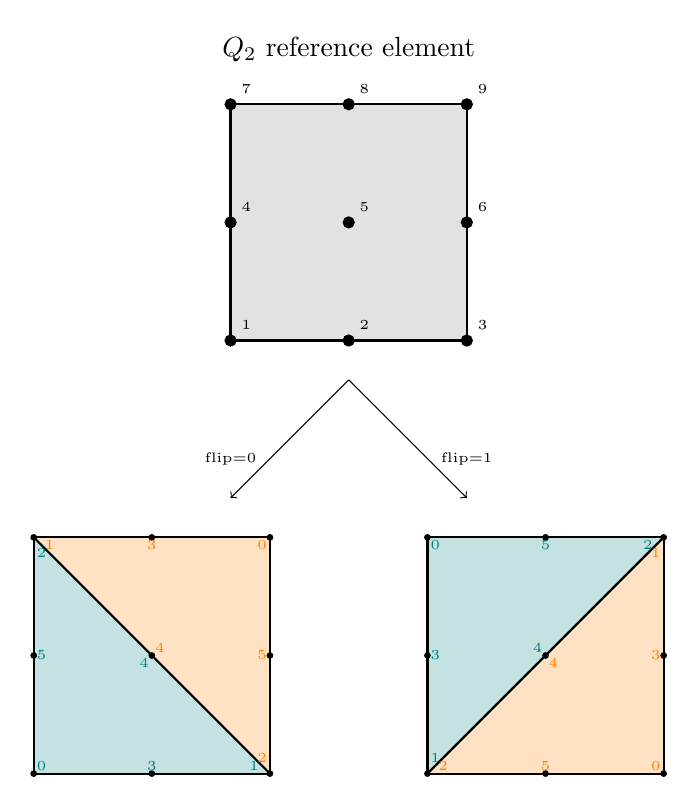
\begin{tikzpicture}
%\draw[fill=gray!23,gray!23](0,0) rectangle (9,10);
%\draw[step=0.5cm,gray,very thin] (0,0) grid (9,10); %background grid

\draw[fill=teal!23,teal!23](0.5,0.5) -- (3.5,0.5) -- (0.5,3.5) -- cycle;
\draw[fill=orange!23,orange!23](3.5,0.5) --(3.5,3.5) -- (0.5,3.5) -- cycle;
\draw[thick] (0.5,0.5) -- (3.5,0.5) -- (3.5,3.5) -- (0.5,3.5) -- cycle; %left
\draw[thick] (0.5,3.5) -- (3.5,0.5) ;
\draw[black,fill=black] (0.5,0.5)   circle (1pt);
\draw[black,fill=black] (2,0.5)   circle (1pt);
\draw[black,fill=black] (3.5,0.5)   circle (1pt);
\draw[black,fill=black] (0.5,2)   circle (1pt);
\draw[black,fill=black] (2,2)   circle (1pt);
\draw[black,fill=black] (3.5,2)   circle (1pt);
\draw[black,fill=black] (0.5,3.5)   circle (1pt);
\draw[black,fill=black] (2,3.5)   circle (1pt);
\draw[black,fill=black] (3.5,3.5)   circle (1pt);
\node[] at (0.6,0.6) {\tiny \color{teal} 0};
\node[] at (2,0.6) {\tiny \color{teal} 3};
\node[] at (3.3,0.6) {\tiny \color{teal} 1};
\node[] at (0.6,2) {\tiny \color{teal} 5};
\node[] at (1.9,1.9) {\tiny \color{teal} 4};
\node[] at (0.6,3.3) {\tiny \color{teal} 2};
\node[] at (3.4,3.4) {\tiny \color{orange} 0};
\node[] at (2,3.4) {\tiny \color{orange} 3};
\node[] at (0.7,3.4) {\tiny \color{orange} 1};
\node[] at (3.4,2) {\tiny \color{orange} 5};
\node[] at (3.4,0.7) {\tiny \color{orange} 2};
\node[] at (2.1,2.1) {\tiny \color{orange} 4};



\draw[fill=teal!23,teal!23](5.5,0.5) -- (8.5,3.5) -- (5.5,3.5) -- cycle;
\draw[fill=orange!23,orange!23](5.5,0.5) --(8.5,0.5) -- (8.5,3.5) -- cycle;

\draw[thick] (5.5,0.5) -- (8.5,0.5) -- (8.5,3.5) -- (5.5,3.5) -- cycle; %right
\draw[thick] (5.5,0.5) -- (8.5,3.5) ;
\draw[black,fill=black] (5.5,0.5)   circle (1pt);
\draw[black,fill=black] (7,0.5)   circle (1pt);
\draw[black,fill=black] (8.5,0.5)   circle (1pt);
\draw[black,fill=black] (5.5,2)   circle (1pt);
\draw[black,fill=black] (7,2)   circle (1pt);
\draw[black,fill=black] (8.5,2)   circle (1pt);
\draw[black,fill=black] (5.5,3.5)   circle (1pt);
\draw[black,fill=black] (7,3.5)   circle (1pt);
\draw[black,fill=black] (8.5,3.5)   circle (1pt);
\node[] at (8.4,0.6) {\tiny \color{orange} 0};
\node[] at (8.4,2) {\tiny \color{orange} 3};
\node[] at (8.4,3.3) {\tiny \color{orange} 1};
\node[] at (7,0.6) {\tiny \color{orange} 5};
\node[] at (7.1,1.9) {\tiny \color{orange} 4};
\node[] at (5.7,0.6) {\tiny \color{orange} 2};

\node[] at (5.6,3.4) {\tiny \color{teal} 0};
\node[] at (5.6,2) {\tiny \color{teal} 3};
\node[] at (5.6,0.7) {\tiny \color{teal} 1};
\node[] at (7,3.4) {\tiny \color{teal} 5};
\node[] at (6.9,2.1) {\tiny \color{teal} 4};
\node[] at (8.3,3.4) {\tiny \color{teal} 2};

\draw[thin,->] (4.5,5.5) -- (3,4); 
\draw[thin,->] (4.5,5.5) -- (6,4); 
\node[] at (3,4.5) {\tiny flip=0};
\node[] at (6,4.5) {\tiny flip=1};

\node[] at (4.5,9.7) {$Q_2$ reference element};
\draw[fill=gray!23,gray!23](3,6) rectangle (6,9);
\draw[thick] (3,6) -- (6,6) -- (6,9) -- (3,9) -- cycle; %top
\draw[black,fill=black] (3,6)   circle (2pt);
\draw[black,fill=black] (4.5,6)   circle (2pt);
\draw[black,fill=black] (6,6)   circle (2pt);
\draw[black,fill=black] (3,7.5)   circle (2pt);
\draw[black,fill=black] (4.5,7.5)   circle (2pt);
\draw[black,fill=black] (6,7.5)   circle (2pt);
\draw[black,fill=black] (3,9)   circle (2pt);
\draw[black,fill=black] (4.5,9)   circle (2pt);
\draw[black,fill=black] (6,9)   circle (2pt);
\node[] at (3.2,6.2) {\tiny 1};
\node[] at (4.7,6.2) {\tiny 2};
\node[] at (6.2,6.2) {\tiny 3};
\node[] at (3.2,7.7) {\tiny 4};
\node[] at (4.7,7.7) {\tiny 5};
\node[] at (6.2,7.7) {\tiny 6};
\node[] at (3.2,9.2) {\tiny 7};
\node[] at (4.7,9.2) {\tiny 8};
\node[] at (6.2,9.2) {\tiny 9};

\end{tikzpicture}


